\hypertarget{main_dialogs}{}
\section{Main dialogs}
\index{Main dialogs}

%% About
%-------------------------------------------------------------------------
\hypertarget{dlg_working_about}{}
\subsection{About}
\index{About}
\index{Main dialogs!About}
\index{About!Project}
\index{About!Aknowledgments}

\begin{figure}[H]
  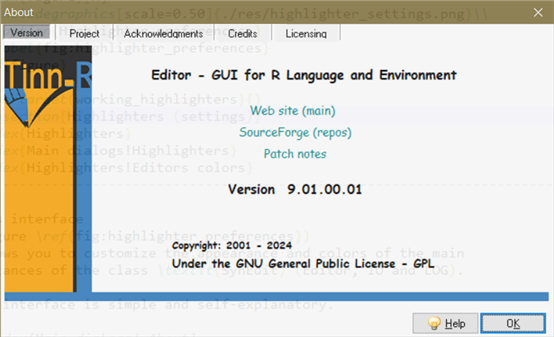
\includegraphics[scale=0.60]{./res/dlg_about.png}~~
  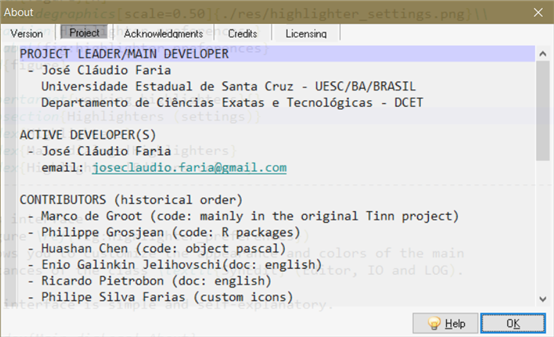
\includegraphics[scale=0.60]{./res/dlg_about_project.png} \\
  \caption{Main screens of the About dialog.}
  \label{fig:dlg_about}
\end{figure}
%-------------------------------------------------------------------------
This dialog
(Figure \ref{fig:dlg_about})
displays generic and important information about the program. The interface is
simple and self-explanatory.


%% ASCII chart
%-------------------------------------------------------------------------
\hypertarget{dlg_ascii_chart}{}
\subsection{ASCII chart}
\index{ASCII chart}
\index{Main dialogs!ASCII chart}
\index{ASCII}

\begin{figure}[H]
  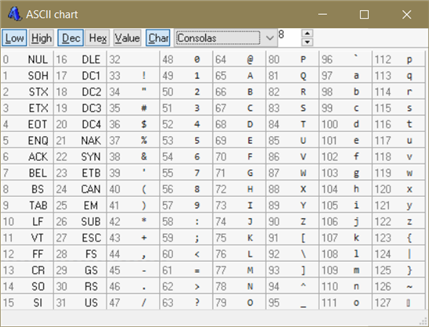
\includegraphics[scale=0.80]{./res/dlg_ascii_chart.png} \\
  \caption{ASCII chart dialog.}
  \label{fig:dlg_ascii_chart}
\end{figure}
%-------------------------------------------------------------------------
This dialog
(Figure \ref{fig:dlg_ascii_chart})
displays a traditional ASCII character table. When you click on a chosen character, it is inserted
into the editor. It's not available - we don't see a need for it - for the \texttt{Term} interface.


%% Card (R)
%-------------------------------------------------------------------------
\hypertarget{dlg_r_card}{}
\subsection{Card (R)}
\index{Card (R)}
\index{Main dialogs!Card (R)}
\index{dataset!card (R)}
\index{database!card (R)}

\begin{figure}[H]
  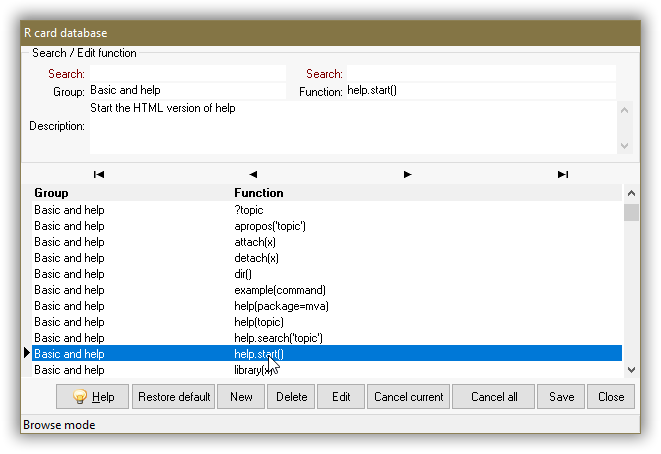
\includegraphics[scale=0.8]{./res/dlg_r_card.png}\\
  \caption{R card (dataset).}
  \label{fig:dlg_r_card}
\end{figure}
%-------------------------------------------------------------------------
The \textit{card} was based on two \RR{} cards already published:
R/Rpad Reference Card by Tom Short and \RR{} reference card by Jonathan Baron.

Read below a brief description of available buttons (Figure \ref{fig:dlg_r_card}):

\begin{quote}
  \begin{footnotesize}
    \begin{description}
      \item[Restore default:]
        Restores the file \texttt{Rcard.xml} from the origin at
        (\texttt{InstallPath/data/data.zip}). Any prior changes in the
        file \texttt{Rcard.xml} currently being used will be lost.
      \item[New:]
        Places the table in insertion mode.
      \item[Delete:]
        Delete the current registry from the table.
      \item[Edit:]
        Places the table in edition mode.
      \item[Cancel current:]
        Cancels any change made to the current edition.
      \item[Cancel all:]
        Cancels all changes made to the database prior to \textit{Save}.
      \item[Save:]
        Overwrites the text file (XML) saving all changes made to the current table.
      \item[Close:]
        Closes the dialog. All non-saved changes will be lost.
    \end{description}
  \end{footnotesize}
\end{quote}


%% Code completion
%-------------------------------------------------------------------------
\hypertarget{dlg_additional_dialogs_code_completion}{}
\subsection{Code completion}
\index{Code completion}
\index{R! Code completion}
\index{Main dialogs!Code completion}
\index{Main dialogs!R code completion}

\begin{figure}[H]
  \begin{center}
    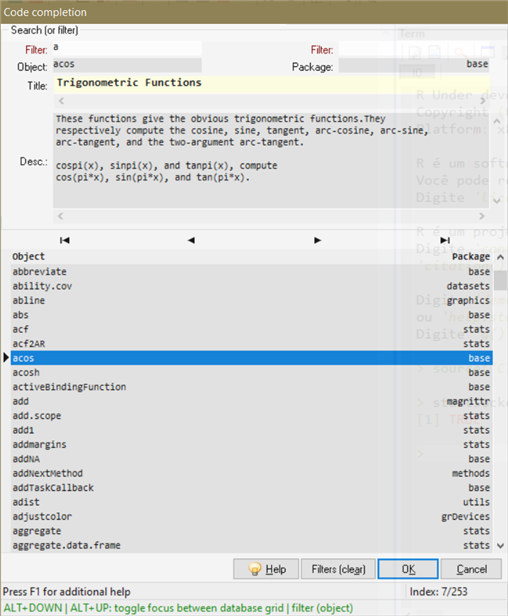
\includegraphics[scale=0.8]{./res/dlg_code_completion.png}
  \end{center}
  \caption{Code completion dialog.}
  \label{fig:dlg_tinn-r_code_completion}
\end{figure}
%-------------------------------------------------------------------------
Code completion
(Figure \ref{fig:dlg_tinn-r_code_completion})
is a dialog window used to search R objects displaying their basic documentation.

The strategy designed for this interface is - in our view - innovative. It is an alternative to what
is conventional in the main IDEs used in programming. These generally try to
guess - with drop-down windows filled with information - what the user wants as they type.
Paradoxically, they are poor in the information needed to make a decision.
In our understanding, drop-down windows generally have a low success rate,
pollute the editing space and do not have features that make it possible to apply filters to
different groups or comfortably browse the options (which in many cases can be 200 or more) in certain cases.

The R code completion dialog window (Figure \ref{fig:dlg_tinn-r_code_completion}) allows you to apply filters
(non-retroactive) to the object name, the package name and allows you to comfortably navigate the dataset
grid seeing as much information as possible about the objects to really enable precise location .

Due to the search mechanism being relatively complex, it was decided not to allow retroactive searches.
In other words, if you don't have detailed information about the object you want to locate in R, the best
option is to start the search with the smallest possible number of characters and apply filters, and/or,
navigate the grid to locate the desired object. In other words, start with a large number and logically
reduce the options until you find what you are looking for.

The shortcuts (ALT+DOWN | ALT+UP) allow you to switch the cursor focus between the editing and filtering
boxes and the datagrid, making it easier to choose the object sought, as a greater amount of documentation
(title and description) is displayed in the interface.

Once located, simply type \texttt{ENTER} (or \texttt{OK}) and the object will be inserted in the Editor,
IO or LOG where the cursor was located when the dialog was called.

Use this dialog as follows:
\begin{enumerate}
  \item Place the cursor where you want to use the code completion
  \item Enter the default shortcut: (\texttt{CTRL+Q}) to open the dialog window
  \item Use edit boxes for object or package filtering
  \item Locate the desired object
  \item ENTER or OK to insert the object
\end{enumerate}

As the search database - however small it is - brings a relatively large volume of information
from the R documentation and is not very fast, searches should only be done progressively
(adding more characters to the initial(s)) in the filter box. In other words, reverse search
is not performed in this interface.


%% Comments
%-------------------------------------------------------------------------
\hypertarget{dlg_working_about}{}
\subsection{Comments}
\index{Comments}
\index{Main dialogs!Comments}
\index{database!comments}
\index{dataset!comments}

\begin{figure}[H]
  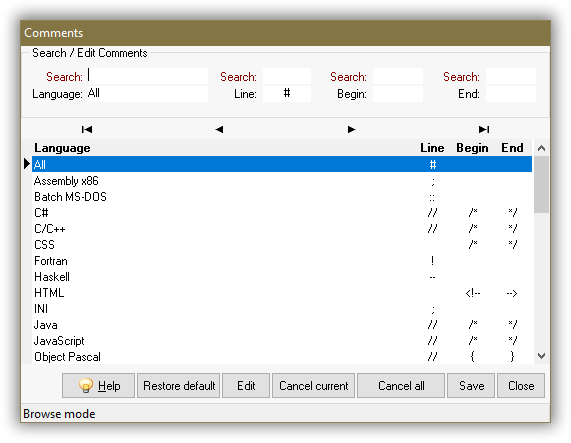
\includegraphics[scale=0.8]{./res/dlg_comments.png}\\
  \caption{Comments (dataset).}
  \label{fig:dlg_comments}
\end{figure}
%-------------------------------------------------------------------------
The \textit{Comments} resource is very simple and allows high level
of user customization.

From version 3.0.1.0 Tinn-R automatically recognizes the
language of the file on focus. Further, inside the file
- if it is a syntax a multi-highlighter (complex syntax) - which language of
the line where the cursor (or selection) is found.

This identification is done automatically if (and only if) the option
\textit{(x) Auto detect language (recomended)} is checked. Otherwise
the user is forcing the application to use the comments of the selected language
(indicator arrow).

Selected code snippets involving more than one language will not be commented/uncommented
and a warning message is issued. That is, you must select only the snippet of a single language.

Read below a brief description of available buttons (Figure \ref{fig:dlg_comments}):

\begin{quote}
  \begin{footnotesize}
    \begin{description}
      \item[Restore default:]
        Restores the file \texttt{Comments.xml} from the origin at
        (\texttt{InstallPath/data/data.zip}). Any prior changes in the
        file \texttt{Comments.xml} currently being used will be lost.
      \item[Edit:]
        Places the table in edition mode.
      \item[Cancel current:]
        Cancels any change made to the current edition.
      \item[Cancel all:]
        Cancels all changes made to the database prior to \textit{Save}.
      \item[Save:]
        Overwrites the text file (XML) saving all changes made to the current table.
      \item[Close:]
        Closes the dialog. All non-saved changes will be lost.
    \end{description}
  \end{footnotesize}
\end{quote}


%% Differences
%-------------------------------------------------------------------------
\hypertarget{dlg_differences}{}
\subsection{Differences}
\index{Differences}
\index{Main dialogs!Differences}

\begin{figure}[H]
  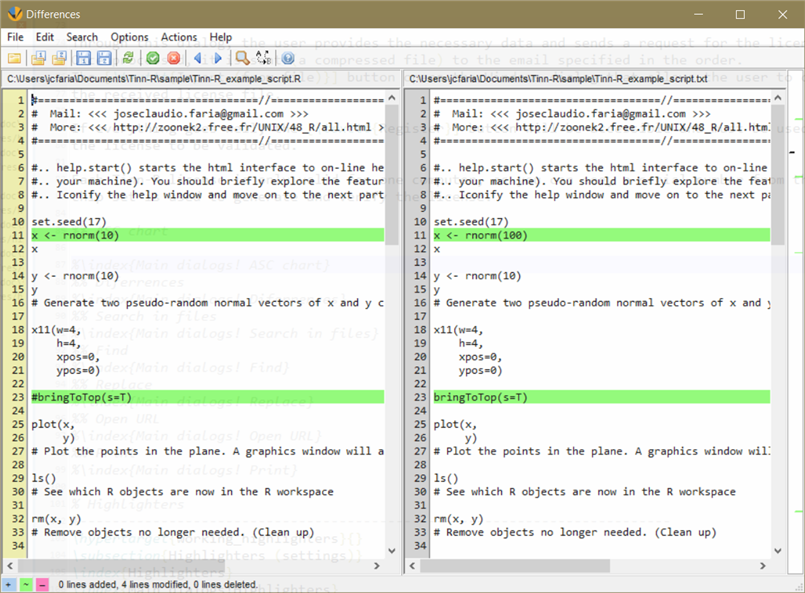
\includegraphics[scale=0.80]{./res/dlg_differences.png} \\
  \caption{Differences dialog.}
  \label{fig:dlg_differences}
\end{figure}
%-------------------------------------------------------------------------
This dialog
(Figure \ref{fig:dlg_differences})
Allows comparison between two directories or between two files.

As it is software developed by third parties - adapted and incorporated into Tinn-R - the documentation
(\texttt{textdiff.hlp}) is in the old Windows documentation system. Therefore, if necessary, you must
install the appropriate Help viewer to read the documentation.

The interface of this dialog is friendly and very intuitive. We are evaluating whether to continue with
this (third-party) application and update the documentation or replace it with something more modern
for the next versions. It - as it is - has served our basic needs well over many years, as it was a
job well done in Object Pascal.


%% Find
%-------------------------------------------------------------------------
\hypertarget{dlg_find}{}
\subsection{Find}
\index{Find}
\index{Main dialogs!Find}

\begin{figure}[H]
  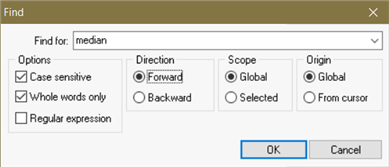
\includegraphics[scale=0.8]{./res/dlg_find.png} \\
  \caption{Find dialog.}
  \label{fig:dlg_find}
\end{figure}
%-------------------------------------------------------------------------
This dialog
(Figure \ref{fig:dlg_find})
and \textit{Replace}
(Figure \ref{fig:dlg_replace})
are very similar.

When you call up the \textit{Find} dialog the \textit{Find for} box will be
prefilled with the word under the cursor. You can type over the entry if you
are looking for another word. There is also a dropdown list of phrases
previously searched.

There are options for Case sensitive, Wole words only, Regular expression,
Direction (Forward an Backward), Scope (Global and Selected) and Origin (Global and From cursor).


%% Highlighters (settings)
%-------------------------------------------------------------------------
\hypertarget{dlg_working_highlighters}{}
\subsection{Highlighters (settings)}
\index{Highlighters}
\index{Main dialogs!Highlighters}
\index{Highlighters!Editors colors}

\begin{figure}[H]
  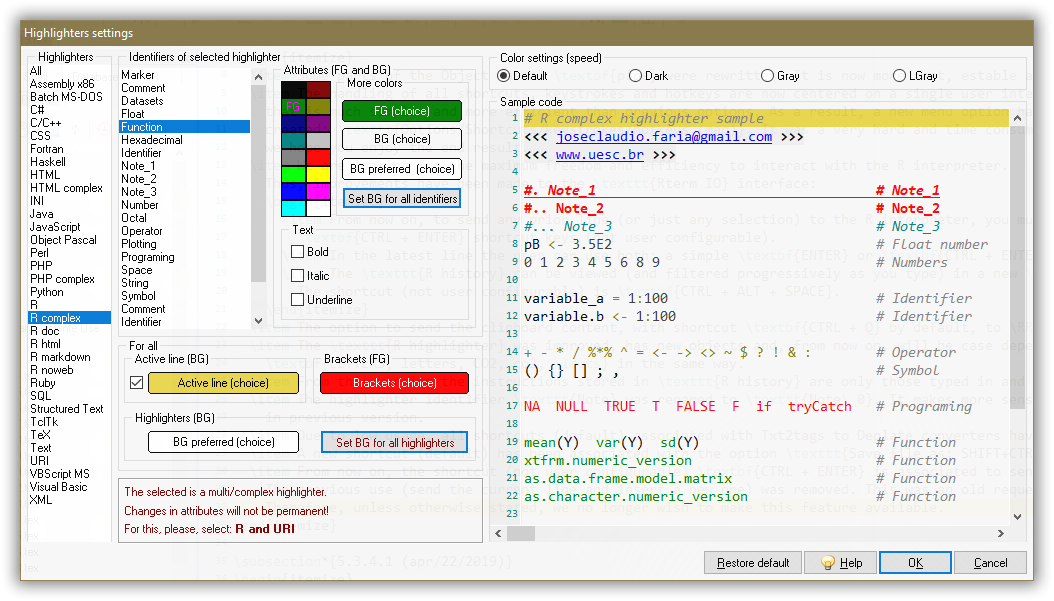
\includegraphics[width=\headwidth]{./res/dlg_highlighter_settings.png}\\
  \caption{Highlighter preferences dialog.}
  \label{fig:dlg_highlighter_preferences}
\end{figure}
%-------------------------------------------------------------------------
This interface
(Figure \ref{fig:dlg_highlighter_preferences})
allows you to customize the appearance and colors of the main
instances of the class \textit{SynEdit} (Editor, IO and LOG).

The interface is simple and self-explanatory.

Basically, make a choice between the set of highlighters available
from the \textit{Highlighters} list. The identifier of the selected
highlighter will be updated. It is possible to set only one
foreground attribute each time. But it is possible to set the
background for all attributes of the selected highlighter and also
the background of all attributes of all highlighters.

It is also possible to set the color brackets and the active line
background.

\subsubsection{Observation:}\\
\index{Highlighters!multi-highlighters}

Tinn-R has seven multi-highlighters: \textit{HTML complex}, \textit{PHP complex},
\textit{R complex}, \textit{R doc},  \textit{R html}, \textit{R markdown} and \textit{R noweb},
with each one behaving as follows:

\begin{footnotesize}
  \begin{verbatim}
    1. HTML complex = HTML & JavaScript
    2. PHP complex  = HTML & JavaScript & PHP
    3. R complex    = R & URI ('<<<' begin URI; '>>>' end URI)
    4. R doc        = TeX & R ('>>=' begin R; '@' end R)
    5. R html       = HTML & R ('<!--begin.rcode' begin R; 'end.rcode-->' end R)
    5. R markdown   = URI & R ('```{' begin R; '```' end R)
    6. R noweb      = TeX & R ('>>=' begin R; '@' end R)

    URI       : Uniform Resource Identifiers.

    R complex : The main syntax is R, '<<<' and '>>>' are the tags enabling
                the user to insert a block of URI syntax.

    R doc     : The main syntax is TeX, '>>=' and '@' are the tags enabling
                the user to insert a block of R syntax.

    R html    : The main syntax is HTML, '<!--begin.rcode' and 'end.rcode-->' are the tags enabling
                the user to insert a block of R syntax.

    R markdown: The main syntax is URI, '```{' and '```' are the tags enabling
                the user to insert a block of R syntax.

    R noweb   : The main syntax is TeX, '>>=' and '@' are the tags enabling
                the user to insert a block of R syntax.
  \end{verbatim}
\end{footnotesize}

These highlighters haven't priorities when you set the syntax color preferences.
Thus, if you change the colors' preferences of any of these multi-highlighters
these settings will be valid only in the current Tinn-R session and will not be
saved when Tinn-R is closed. So, if you want to make permanent changes, set the
preferences from all simple highlighters.

From version 3.0.1.0 a warning message is displayed whenever
a multi-highlighter is selected. It shows which highlighters the user
must change the characteristics so that they are properly stored and
henceforth always displayed.


%% Hotkeys (Send/Control/Custom)
%-------------------------------------------------------------------------
\hypertarget{dlg_hotkeys_editor}{}
\subsection{Hotkeys (Send/Control/Custom)}
\index{Hotkeys!Send}
\index{Hotkeys!Control}
\index{Hotkeys!Custom}
\index{database!hotkeys}
\index{dataset!Hotkeys (Send)}
\index{dataset!Hotkeys (Control)}
\index{dataset!Hotkeys (Custom)}

\begin{figure}[H]
  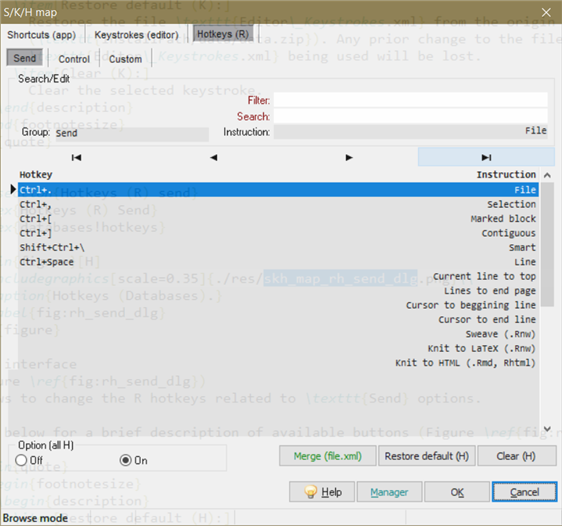
\includegraphics[scale=0.6]{./res/dlg_skh_map_rh_send.png}~~
  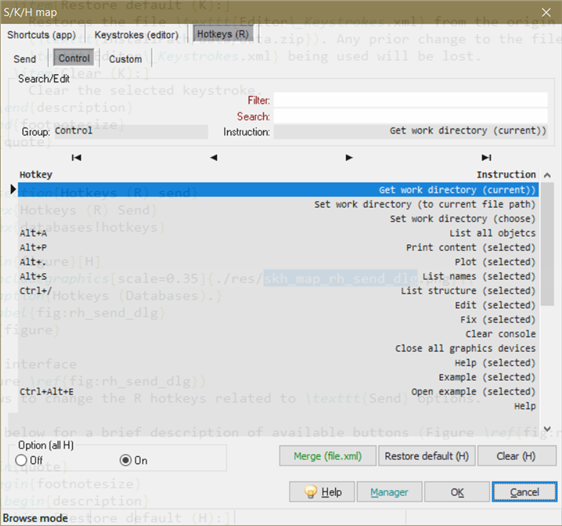
\includegraphics[scale=0.6]{./res/dlg_skh_map_rh_control.png}\\
  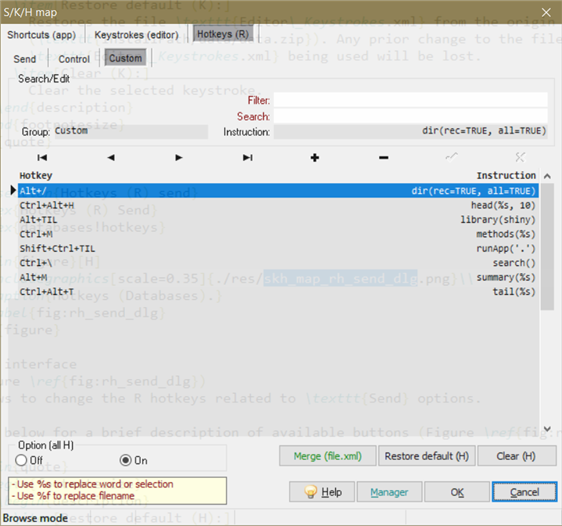
\includegraphics[scale=0.6]{./res/dlg_skh_map_rh_custom.png}\\
  \caption{Hotkeys (database).}
  \label{fig:dlg_skh_map_hotkeys}
\end{figure}
%-------------------------------------------------------------------------

The \textit{Hotkeys (operational system)}
(Figure \ref{fig:dlg_skh_map_hotkeys})
allow setting the hotkeys
related to the operational system. The difference between those hotkeys and
\textit{Shortcuts customization} is that the latter works only with the
focus in Tinn-R, whereas the hotkeys work with the focus anywhere.

The interface is self-explanatory. Basically you first make a choice from
the \textit{R/Hotkeys (operational system)} and set the desired Hotkey.

The set of hotkeys will perform actions only if the option \textit{Active}
is checked. The objective of these options (\textit{Inactive} and
\textit{Active}) is to avoid conflict with others applications allowing
to enable/disable the set of hotkeys quickly and easily.

The \texttt{R/Hotkeys} interface was deeply reworked in the version 5.05.01.01 and it now has three tabs,
\texttt{Send}, \texttt{Control} and \texttt{Custom}:

\begin{itemize}
\item \texttt{Send}: Contains the already traditional \texttt{Send} instructions of Tinn-R;
\item \texttt{Custom}: Contains the already traditional \texttt{Control} instructions of Tinn-R;
\item \texttt{Custom}: \textbf{Allows the user to customize any instructions} to be send to \RR{} interpreter (thanks to Philemon Lenherr for the suggestion). The instructions must be as follows:
 \begin{itemize}
 \item Simple: \texttt{search()}. The \RR{} interpreter will receive \texttt{$>$ search()};
 \item Replace word or small selection: \texttt{View(\%s, title='View of iris dataset')}.
   If the editor cursor is over the word \texttt{iris} or it is selected,
   the \RR{} interpreter will receive \texttt{$>$ View(iris, title='View of iris dataset')}
 \item Replace whole file: \texttt{source(\%f, echo=TRUE, verbose=TRUE)}.
   The \RR{} interpreter will receive \texttt{$>$ source(.trPaths[4], echo=TRUE, verbose=TRUE)}.
   All rules related to send file are preserved.
 \end{itemize}
\end{itemize}

Starting with version 5.05.01.01, the number of \texttt{Custom} statements the user can define is unlimited.


%% Keystrokes (Editor)
%-------------------------------------------------------------------------
\hypertarget{dlg_keystrokes_editor}{}
\subsection{Keystrokes (Editor)}
\index{Keystrokes (Editor)}
\index{Main dialogs!Keystrokes (Editor)}
\index{editor!keystrokes}
\index{database!Keystrokes (Editor)}
\index{dataset!Keystrokes (Editor)}

\begin{figure}[H]
  \begin{center}
    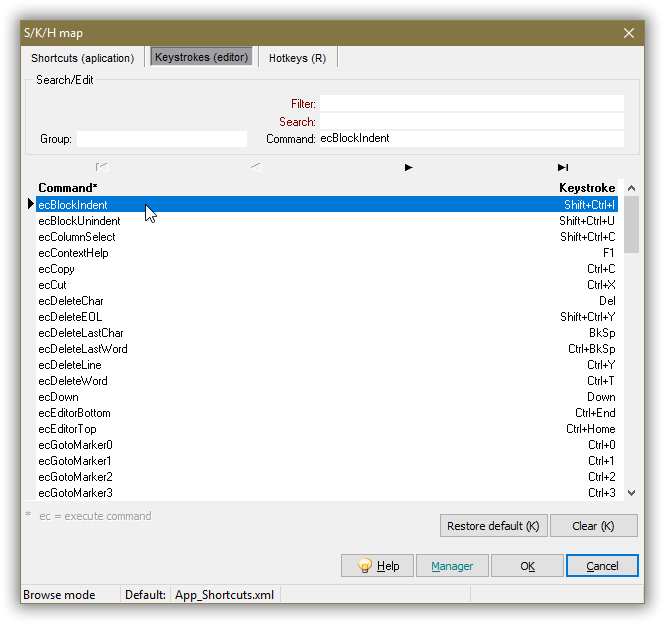
\includegraphics[scale=0.8]{./res/dlg_skh_map_keystrokes.png}\\
  \end{center}
  \caption{Keystrokes (dataset).}
  \label{fig:dlg_skh_map_keystrokes}
\end{figure}
%-------------------------------------------------------------------------

This interface
(Figure \ref{fig:dlg_skh_map_keystrokes})
allows to change the default SynEdit keystrokes.
It is possible only change the keystroke associaed to any \texttt{ecAction} (execute command action).
A set of user friendly keystrokes gives high productivity leading with
all instances of the class \textit{SynEdit}: Editor, IO and LOG.

Read below for a brief description of available buttons (Figure \ref{fig:dlg_skh_map_keystrokes}):

\begin{quote}
  \begin{footnotesize}
    \begin{description}
      \item[Restore default (K):]
        Restores the file \texttt{Editor\_Keystrokes.xml} from the origin at
        (\texttt{InstallPath/data/data.zip}). Any prior change to the file ini file
        \texttt{Editor\_Keystrokes.xml} being used will be lost.
      \item[Clear (K):]
        Clear the selected keystroke.
    \end{description}
  \end{footnotesize}
\end{quote}


%% License manager
%-------------------------------------------------------------------------
\hypertarget{dlg_license_manager}{}
\subsection{License manager}
\index{License manager}
\index{Main dialogs!License manager}

\begin{figure}[H]
  \begin{center}
    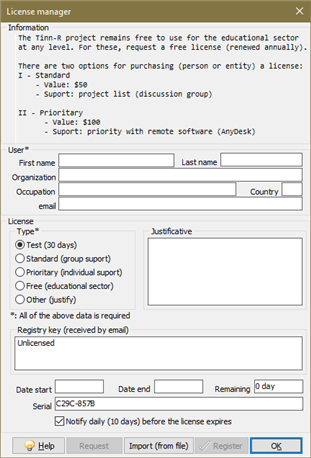
\includegraphics[scale=0.8]{./res/dlg_license_manager.png}\\
  \end{center}
  \caption{License manager.}
  \label{fig:dlg_license_manager}
\end{figure}
%-------------------------------------------------------------------------

This interface
(Figure \ref{fig:dlg_license_manager})
allows the license manager dialog.

This dialog must be used to manage program licenses. There you can request \texttt{[Request]},
Import \texttt{[Import (from file)]} and Register \texttt{[Register]} the usage license.

All use licenses are valid for one year from the date of issue.

Tinn-R does not restrict any of its features, even for unlicensed versions. However, at each period of
time determined by the developers, the user with an unlicensed version (or an expired version) observes
an informative dialog about licensing on their monitor screen.


%% Mirrors (R)
%-------------------------------------------------------------------------
\hypertarget{dlg_mirrors}{}
\subsection{Mirrors (R)}
\index{Mirrors}
\index{Main dialogs!Mirrors}
\index{database!mirrors (R)}
\index{dataset!mirrors (R)}

\begin{figure}[H]
  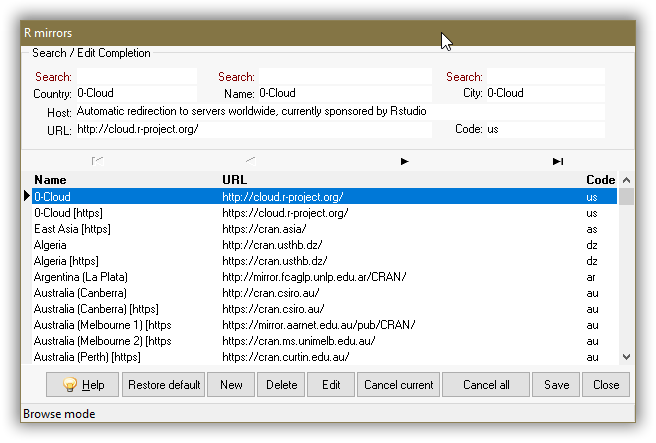
\includegraphics[scale=0.8]{./res/dlg_mirrors.png}\\
  \caption{R mirrors (dataset).}
  \label{fig:dlg_mirrors}
\end{figure}
%-------------------------------------------------------------------------
The \textit{Mirrors} is an interface that allows the user to manage the
repositories (or mirrors) of \RR{}.

You should always choose a repository physically closest to where you are,
so that, the Web communication tends to be faster and more efficient.

The default mirror is the University \href{http://cran.at.r-project.org/}{Wien}
(Austria). Consider that this is the central mirror of CRAN.

The reasons for the Tinn-R always set a repository are two:
\begin {itemize}
   \item Prevent \RR{} keep asking which repository you want to use in each session;
   \item Workaround of intermittency (only Rterm.exe) display the dialog for selecting the repository.
    That is, sometimes the dialog is displayed and not others.
    The cause of this intermittency is still unknown.
\end {itemize}

Read below a brief description of available buttons (Figure \ref{fig:dlg_mirrors}):

\begin{quote}
  \begin{footnotesize}
    \begin{description}
      \item[Restore default:]
        Restores the file \texttt{Rmirrors.xml} from the origin at
        (\texttt{InstallPath/data/data.zip}). Any prior change to the
        file \texttt{Rmirrors.xml} while being used will be lost.
      \item[New:]
        Places the table in insertion mode.
      \item[Delete:]
        Deletes the current registry from the table.
      \item[Edit:]
        Places the table in edition mode.
      \item[Cancel current:]
        Cancels any change made during the current editing session.
      \item[Cancel all:]
        Cancels all changes made to the database prior to \textit{Save}.
      \item[Save:]
        Overwrites the text file (XML) while saving all changes made to the current table.
      \item[Close:]
        Closes the dialog. All changes not previously saved will be lost.
    \end{description}
  \end{footnotesize}
\end{quote}


%% Open URL
%-------------------------------------------------------------------------
\hypertarget{dlg_open_url}{}
\subsection{Open URL}
\index{Open URL}
\index{Main dialogs!Open URL}

\begin{figure}[H]
  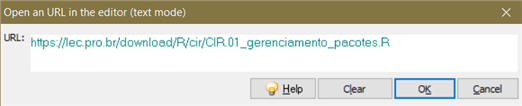
\includegraphics[scale=1]{./res/dlg_open_url.png} \\
  \caption{Open URL dialog.}
  \label{fig:dlg_open_url}
\end{figure}
%-------------------------------------------------------------------------
This dialog
(Figure \ref{fig:dlg_open_url})
allows the user to inform a Uniform Resource Locator (URL) of a file available on the WEB
that they want to open in Tinn-R for viewing and/or editing.

A copy of the file saved and opened in the operating system's temporary folder
with a suffix added to its name \texttt{[hh\_mm\_ss]} to make it unique. If desired,
the user can use the Save as option, choose a more suitable location to
store it and remove the suffix to simplify the file name.


%% Pandoc
%-------------------------------------------------------------------------
\hypertarget{dlg_working_pandoc}{}
\subsection{Pandoc}
\index{Pandoc}
\index{Main dialogs!Pandoc}

\begin{figure}[H]
  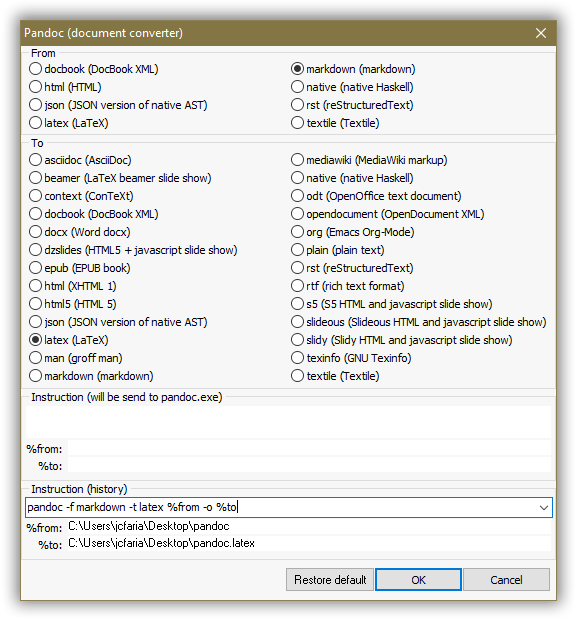
\includegraphics[scale=0.8]{./res/pandoc.png} \\
  \caption{Pandoc (document converter).}
  \label{fig:dlg_pandoc}
\end{figure}
%-------------------------------------------------------------------------
This dialog
(Figure \ref{fig:dlg_pandoc})
displays a simple GUI made to make more easy to convert files from one markup format into another using
\href{https://pandoc.org/index.html}{Pandoc}. The interface is simple and self-explanatory.
Be aware that Pandoc requires that the file to be converted is in UTF-8 format.


%% Print
%-------------------------------------------------------------------------
\hypertarget{dlg_print}{}
\subsection{Print}
\index{Print}
\index{Main dialogs!Print}

\begin{figure}[H]
  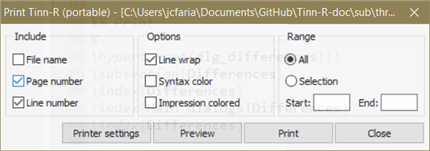
\includegraphics[scale=1]{./res/dlg_print.png} \\
  \caption{Print dialog.}
  \label{fig:dlg_print}
\end{figure}
%-------------------------------------------------------------------------
This dialog
(Figure \ref{fig:dlg_print})
allows the user to define the main options related to printing the active document.
It also allows you to define the printer properties \texttt{[Printer settings]},
see in advance how the print will be \texttt{[Preview]},
print directly if you have already defined the preferences and close the dialog \texttt{[Close]}.


%% Print preview
%-------------------------------------------------------------------------
\hypertarget{dlg_print_preview}{}
\subsection{Print preview}
\index{Print preview}
\index{Main dialogs!Print preview}

\begin{figure}[H]
  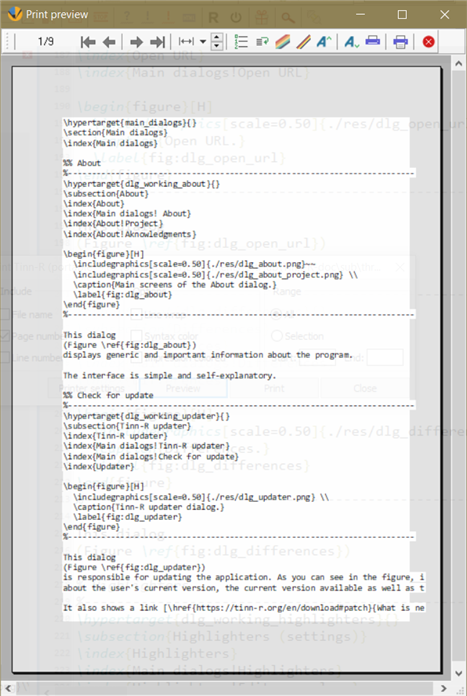
\includegraphics[scale=0.8]{./res/dlg_print_preview.png} \\
  \caption{Print preview dialog.}
  \label{fig:dlg_print_preview}
\end{figure}
%-------------------------------------------------------------------------
This dialog
(Figure \ref{fig:dlg_print_preview})
is opened - at the user's option - if they want to see in advance what the printout of
the open document will look like.

It is a simple interface that allows you to define or reset printer and printing properties.


%% Find and Replace
%-------------------------------------------------------------------------
\hypertarget{find_replace}{}
\subsection{Find and replace}
\index{find}
\index{replace}

\subsubsection{Find:}\\
\index{find}
\begin{figure}[H]
  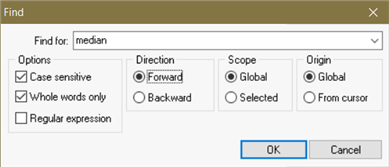
\includegraphics[scale=1]{./res/dlg_find.png}\\
  \caption{Find dialog.}
  \label{fig:dlg_find}
\end{figure}
%-------------------------------------------------------------------------

The dialogs for \textit{Find}
and \textit{Replace}
(Figure \ref{fig:dlg_find} and \ref{fig:dlg_replace})
are very similar, so this session will just discuss the \textit{Replace} dialog
and will point out the changes when necessary.

When you call up the \textit{Find} dialog
the \textit{Find for} box will be
prefilled with the word under the cursor. You can type over the entry if you
are looking for another word. There is also a dropdown list of phrases
previously searched.


\subsubsection{Replace:} \\
\index{replace}
\begin{figure}[H]
  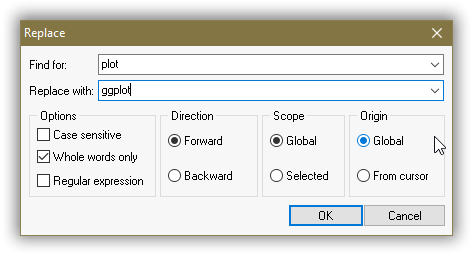
\includegraphics[scale=1]{./res/dlg_replace.png}\\
  \caption{Find and replace dialog.}
  \label{fig:dlg_replace}
\end{figure}

When you call up the \textit{Replace} dialog
(Figure \ref{fig:dlg_replace})
the \textit{Replace with} box
will be filled with the last string you entered in it. If this is the first
time you have called the \textit{Replace} dialog since starting Tinn-R then
the Replace box will be empty. You can type over any text in box. There is
also a dropdown list of strings previously used.

\subsubsection{Options:}\\
\begin{quote}
  \begin{footnotesize}
    \begin{description}
      \item[Case sensitive:]
        When this option is set the search is done case sensitively. For instance,
        \texttt{Ab}, \texttt{AB} and \texttt{ab} are all treated as different words
        whereas they are not if the option is not set.
      \item[Whole words only:]
        When this option is set the system will only find complete words matching
        the search criteria. So, for example, if \texttt{ab} is the search string
        the system will not match occurrences of words like \texttt{abc} or
        \texttt{cab}.
      \item[Regular expressions:]
        \href{\#working\_regularexpressions}{See regular expressions ...}
    \end{description}
  \end{footnotesize}
\end{quote}


\subsubsection{Direction:}\\
The direction to search. This option is ignored if searching in selected text.

\begin{quote}
  \begin{footnotesize}
    \begin{description}
      \item[Forward:]
        Search from the cursor position to the end of the file.
      \item[Backward:]
        Search from the cursor position to the beginning of the file.
    \end{description}
  \end{footnotesize}
\end{quote}

\subsubsection{Scope:}\\
\begin{quote}
  \begin{footnotesize}
    \begin{description}
      \item[Global:]
        Search the entire file.
      \item[Selected Text:]
        Search just the selected text.
    \end{description}
  \end{footnotesize}
\end{quote}

\subsubsection{Origin:}\\
\begin{quote}
  \begin{footnotesize}
    \begin{description}
      \item[Global:]
        Search from the beginning of the file.
      \item[From cursor:]
        Search just from the position of the cursor.
    \end{description}
  \end{footnotesize}
\end{quote}


%% Search in files
%-------------------------------------------------------------------------
\hypertarget{dlg_search_in_files}{}
\subsection{Search in files}
\index{Search in files}
\index{Main dialogs!Search in files}

\begin{figure}[H]
  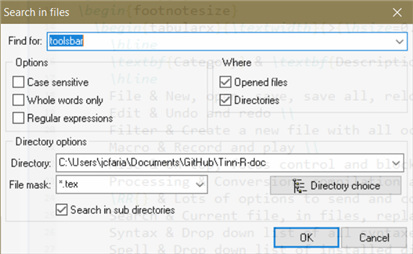
\includegraphics[scale=0.8]{./res/dlg_search_in_files.png}~~
  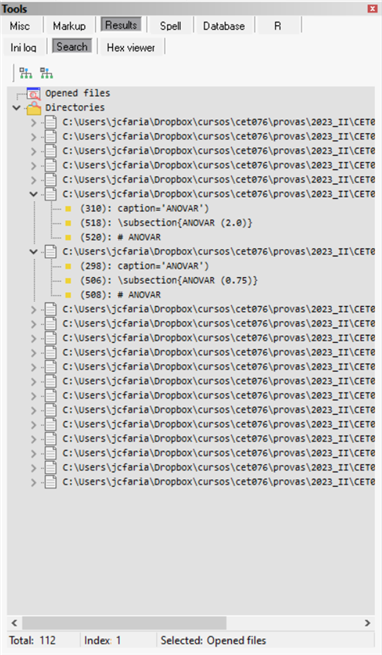
\includegraphics[scale=0.8]{./res/tools_results_search.png}\\
  \caption{Search in files dialog.}
  \label{fig:dlg_search_in_files}
\end{figure}
%-------------------------------------------------------------------------
This dialog
(Figure \ref{fig:dlg_search_in_files})
allows you to match a criteria in all opened files and/or in files on disk.

\subsubsection{Options:}\\
\index{search!case sensitivity}
\index{search!regular expressions}

\begin{quote}
  \begin{footnotesize}
    \begin{description}
      \item[Case sensitive:]
        When this option is set the search is case sensitive.
        For example, \texttt{Ab}, \texttt{AB} and \texttt{ab}
        are all treated as different words.
      \item[Whole words only:]
        When this option is set the system will only find complete
        words matching the search criteria. For example, if
        \texttt{ab} is the search string the system will not match
        occurrences of words such as \texttt{abc} or \texttt{cab}.
      \item[Regular expressions:]
        \href{\#working\_regularexpressions}{See regular expressions ...}
    \end{description}
  \end{footnotesize}
\end{quote}

\subsubsection{Where:}\\

\begin{quote}
  \begin{footnotesize}
    \begin{description}
      \item[Opened files:]
        When this option is set the search is performed on all opened files.
      \item[Directories:]
        When this option is set the search is performed in disk files.
    \end{description}
  \end{footnotesize}
\end{quote}

\subsubsection{Directory options:}\\

\begin{quote}
  \begin{footnotesize}
    \begin{description}
      \item[Directory:]
        A dropdown list of previously searched directories.
      \item[File mask:]
        A dropdown list of the previously searched file mask.
      \item[Search in sub directories:]
        When this option is set the search is performed on all sub
        directories of the main directory.
    \end{description}
  \end{footnotesize}
\end{quote}

\subsubsection{Results interface:}\\
\index{search!results}

The associated results interface
(Figure \ref{fig:search_in_files})
shows the results.

A double click in a single occurrence (or dragging and dropping it into the
editor interface) will open the file and results will be placed in the first
line of the editor window.


%% Search (trigger|snippet)
%-------------------------------------------------------------------------
\hypertarget{dlg_additional_dialogs_search_trigger}{}
\subsection{Search (trigger|snippet)}
\index{Snippet}
\index{Main dialogs!Search snippet}

\begin{figure}[H]
  \begin{center}
    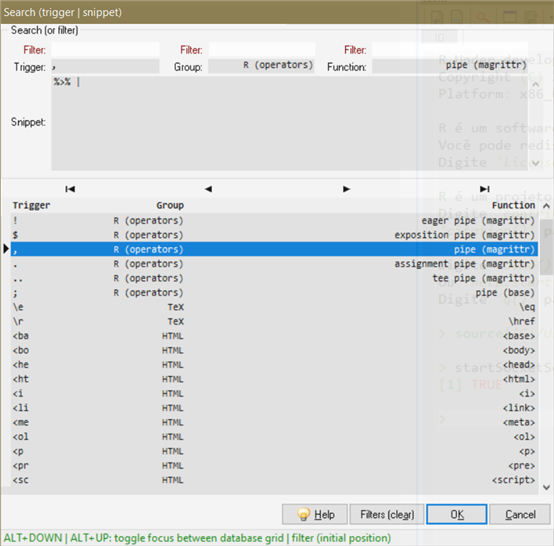
\includegraphics[scale=0.80]{./res/dlg_search_trigger_snippet.png}
  \end{center}
  \caption{Search (trigger|snippets) dialog.}
  \label{fig:dlg_tinn-r_search_trigger}
\end{figure}
%-------------------------------------------------------------------------
Snippets
(Figure \ref{fig:dlg_tinn-r_search_trigger})
are a way to efficiently edit previously-formed, frequently used blocks of text.

As the user creates personalized snippets (and associated triggers) in the database,
it can become difficult to remember all the triggers.
This dialog - Search (trigger|snippet) - (Figure \ref{fig:dlg_tinn-r_search_trigger}) is intended
to make it easier to find the trigger, if users don't remember it.

Allows you to filter table occurrences by trigger, group and function, individually or simultaneously.

The shortcuts (ALT+DOWN | ALT+UP) allow you to switch the cursor focus between the editing and
filtering boxes and the datagrid, making it easier to choose the trigger associated with the snippet.

Once located, simply type \texttt{ENTER} (or \texttt{OK}) and the trigger will be inserted in the Editor,
IO or LOG where the cursor was located when the dialog was called.

What happens next is dependent on a user option: \texttt{Options/Insert code snippet (after trigger search or insertion from DB)}.
If it is not selected, only the trigger will be inserted and the user needs to fire the
trigger (\texttt{CTRL+J}) - by default - for the snippet to be inserted in place of the trigger.
If the above option is checked, the trigger will be inserted followed by the snippet.
In both cases (\texttt{CTRL+Z}) undoes what was done.

Use this dialog as follows:
\begin{enumerate}
  \item Place the cursor where you want to insert a snippet
  \item Enter the default shortcut: (\texttt{SHIFT+CTRL+Q}) to open the dialog window
  \item Use edit boxes for trigger/snippet filtering
  \item Locate the desired trigger/snippet
  \item ENTER or OK to insert the trigger
\end{enumerate}

As the search database - however large it may be - is relatively small and the search and filtering
mechanism is very fast, searches can be made progressive (adding more characters to the initial(s))
or retroactive (completely changing content) in the trigger filter box.


%% Shortcuts (Application)
%-------------------------------------------------------------------------
\hypertarget{dlg_skh_map_shortcuts}{}
\subsection{Shortcuts (Application)}
\index{Shortcuts (Application)}
\index{Main dialogs!Shortcuts (Application)}
\index{database!Shortcuts (Application)}
\index{dataset!Shortcuts (Application)}

\begin{figure}[H]
  \begin{center}
    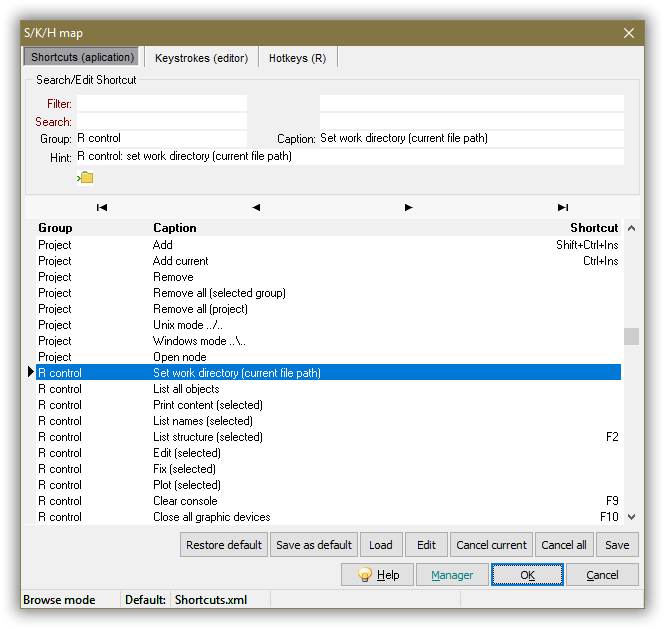
\includegraphics[scale=0.8]{./res/dlg_skh_map_shortcuts.png}\\
  \end{center}
  \caption{Shortcuts (app) (dataset)).}
  \label{fig:dlg_shortcuts}
\end{figure}
%-------------------------------------------------------------------------
The \textit{Shortcuts (app)}
(Figure \ref{fig:dlg_shortcuts})
allows the user to set the shortcuts related
to the application, it works together with the \textit{Editor keystrokes},
and allows for high level of customization.

The difference between \textit{Shortcuts} and \textit{Hotkeys (operational system)}
is that the former works only with the focus on Tinn-R, whereas hotkeys work
with the focus anywhere.

Read below a brief description of available buttons.

\begin{quote}
  \begin{footnotesize}
    \begin{description}
      \item[Restore default:]
        Restores the file \texttt{Shortcuts.xml} from the origin
        (InstallPath/data/data.zip). Any prior changes to the file
        \texttt{Shortcuts.xml} in use will be lost.
      \item[Save as default:]
        Opens the save dialog allowing to save the file. From this
        point, this file will be the new default shortcuts.
      \item[Load:]
        Opens the open dialog allowing to load a shortcut file. From this
        point on, this file will be the new default shortcuts.
      \item[Edit:]
        Sets the table in edition mode.
      \item[Cancel current:]
        Cancels any changes made to the current edition.
      \item[Cancel all:]
        Cancels all changes made to the database prior to \textit{Save}
        or \textit{Save as default}.
      \item[Save:]
        Saves to text file (XML) all changes made to the current table.
      \item[Close:]
        Closes the dialog. All changes not saved will be lost.
    \end{description}
  \end{footnotesize}
\end{quote}


%% S/K/H manager
%-------------------------------------------------------------------------
\hypertarget{dlg_skh_manager}{}
\subsection{S/K/H manager}
\index{S/K/H manager}
\index{Main dialogs!S/K/H manager}

\begin{figure}[H]
  \begin{center}
    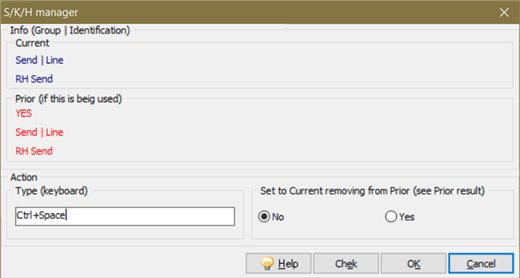
\includegraphics[scale=0.8]{./res/dlg_skh_manager.png}
  \end{center}
  \caption{S/K/H manager.}
  \label{fig:dlg_skh_manager}
\end{figure}
%-------------------------------------------------------------------------
S/K/H manager
(Figure \ref{fig:dlg_skh_manager})
is the dialog responsible for checking, replacing and assigning shortcuts to the application itself,
through the \texttt{SynEdit} class instances (editor, Term/IO and Term/LOG) and also through the hotkeys
associated with R: send, control and custom.

In other words, it is the dialog that centralizes the checks and assignments of shortcuts and hotkeys.
Access to it is via the \texttt{[Manager]} button in the S/K/H map dialog
((Figure \ref{fig:dlg_skh_map_shortcuts},
         \ref{fig:dlg_skh_map_keystrokes} and
         \ref{fig:dlg_skh_map_hotkeys})).


%% Snippets
%-------------------------------------------------------------------------
\hypertarget{snippets}{}
\subsection{Snippets}
\index{snippets}
\index{editor!snippets}
\index{database!snippets}
\index{dataset!snippets}

\begin{figure}[H]
  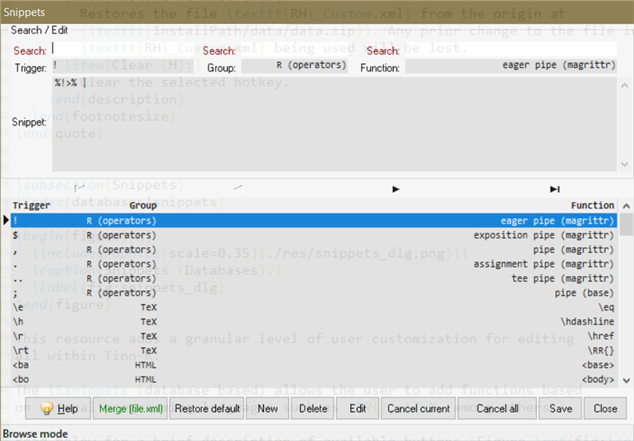
\includegraphics[scale=.8]{./res/dlg_snippets.png}\\
  \caption{Snippets (dataset).}
  \label{fig:dlg_snippets}
\end{figure}
%-------------------------------------------------------------------------
This interface
(Figure \ref{fig:dlg_snippets})
allows to change the default SynEdit keystrokes.
It is possible only change the keystroke associaed to any \texttt{ecAction} (execute command action).
A set of user friendly keystrokes gives high productivity leading with
all instances of the class \textit{SynEdit}: Editor, IO and LOG.

Read below for a brief description of available buttons (Figure \ref{fig:keystrokes_dlg}):

\begin{quote}
  \begin{footnotesize}
    \begin{description}
      \item[Restore default (K):]
        Restores the file \texttt{Editor\_Keystrokes.xml} from the origin at
        (\texttt{InstallPath/data/data.zip}). Any prior change to the file ini file
        \texttt{Editor\_Keystrokes.xml} being used will be lost.
      \item[Clear (K):]
        Clear the selected keystroke.
    \end{description}
  \end{footnotesize}
\end{quote}

\texttt{Tools/Completion} has been replaced by \texttt{Tools/Snippets}. The \texttt{Completion.xml}
table is now named \texttt{Snippets.xml}. Users who have made (and saved) an extensive dataset of completion
(before) (snippets from now on) will be able to notice a new button [\texttt{Merge (file .xml)}] that has been added
in the new \texttt{Snippets} dialog window. When a new dataset (or any update to the source) is made,
the user's dataset (\texttt{Completion.xml} or \texttt{Snippet.xml}, respectively) is saved in the \textbf{bkp} folder which is located
in the Tinn-R startup folders (\texttt{Help/Ini files (path information)}). The new button allows the user's old base
(completion or snippets) to be merged with the current one distributed with the new versions and eventually
modified at the source. Thanks to Ivan B. Allaman for the helpful suggestion.


%% Tinn-R updater
%-------------------------------------------------------------------------
\hypertarget{dlg_working_updater}{}
\subsection{Tinn-R updater}
\index{Tinn-R updater}
\index{Main dialogs!Tinn-R updater}
\index{Main dialogs!Check for update}
\index{Updater}

\begin{figure}[H]
  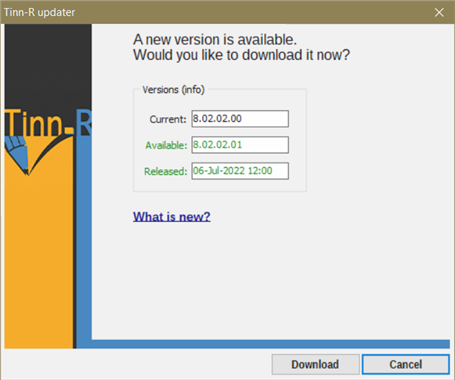
\includegraphics[scale=1]{./res/dlg_updater.png} \\
  \caption{Tinn-R updater dialog.}
  \label{fig:dlg_updater}
\end{figure}
%-------------------------------------------------------------------------
This dialog
(Figure \ref{fig:dlg_updater})
is responsible for updating the application. As you can see in the figure, information is displayed
about the user's current version, the current version available as well as the date of its release.

It also shows a link [\href{https://tinn-r.org/en/download#patch}{What is new?}] so that the user can read the new features implemented on the
project website and decide whether to update or not.

The [\texttt{DOMLOAD}] button starts the update process, just follow the subsequent instructions for the program
to be updated.
